% !TEX program = xelatex
\documentclass[UTF8,zihao=-4,oneside,openany]{ctexbook}
% Shared style for the combined handout.  Section files keep standalone
% preambles for now, while the master document uses this single definition.
\usepackage[a4paper,top=20mm,bottom=22mm,left=19mm,right=19mm,headheight=24pt]{geometry}
\usepackage[table]{xcolor}
\usepackage{amsmath,amssymb,mathtools,bm}
\usepackage{siunitx}
\usepackage{booktabs,tabularx,array,multicol}
\usepackage{enumitem}
\usepackage{tikz}
\usetikzlibrary{arrows.meta,positioning,calc,angles,quotes,patterns}
\usepackage[most]{tcolorbox}
\usepackage{fancyhdr}
\usepackage{hyperref}

\definecolor{Ink}{HTML}{202326}
\definecolor{DeepBlue}{HTML}{294E69}
\definecolor{Blue}{HTML}{47687D}
\definecolor{PaleBlue}{HTML}{F3F5F6}
\definecolor{Gold}{HTML}{6E777D}
\definecolor{PaleGold}{HTML}{F6F6F5}
\definecolor{Green}{HTML}{5B6D76}
\definecolor{PaleGreen}{HTML}{F3F5F6}
\definecolor{Alert}{HTML}{666B6F}
\definecolor{PaleAlert}{HTML}{F6F6F6}
\definecolor{RuleGray}{HTML}{D3D7DA}
\definecolor{TextGray}{HTML}{61686D}
\definecolor{SoftGray}{HTML}{F6F6F6}

\color{Ink}
\sisetup{
  per-mode=symbol,
  inter-unit-product=\ensuremath{{}\cdot{}},
  exponent-product=\times
}

\hypersetup{
  colorlinks=true,
  linkcolor=DeepBlue,
  urlcolor=Blue,
  pdfsubject={高中物理竞赛一轮资料重排讲义},
  pdfauthor={物理竞赛一轮资料编写组}
}

\setlength{\parindent}{2em}
\setlength{\parskip}{0.25em}
\setlist{nosep,leftmargin=2em}
\setcounter{secnumdepth}{3}
\setcounter{tocdepth}{2}
\numberwithin{equation}{section}
\counterwithin{table}{section}
\allowdisplaybreaks[2]
\emergencystretch=2em

\ctexset{
  chapter={
    format=\raggedright\LARGE\bfseries\color{Ink},
    titleformat=\LARGE\bfseries\color{Ink},
    beforeskip=0pt,
    afterskip=18pt
  },
  section={
    format=\Large\bfseries\color{DeepBlue},
    beforeskip=1.8ex,
    afterskip=1.0ex
  },
  subsection={
    format=\large\bfseries\color{Ink},
    beforeskip=1.5ex,
    afterskip=0.8ex
  },
  subsubsection={format=\normalsize\bfseries\color{Ink}}
}

\pagestyle{fancy}
\fancyhf{}
\fancyhead[L]{\small\color{TextGray}高中物理竞赛一轮讲义}
\fancyhead[R]{\small\color{TextGray}第一章\quad 数学与物理工具}
\fancyfoot[C]{\small\color{TextGray}\thepage}
\renewcommand{\headrulewidth}{0.4pt}
\renewcommand{\headrule}{\hbox to\headwidth{\color{RuleGray}\leaders\hrule height \headrulewidth\hfill}}

\newcommand{\dimens}[1]{\operatorname{dim}\!\left(#1\right)}
\newcommand{\dd}{\mathop{}\!\mathrm{d}}
\newcommand{\vect}[1]{\bm{#1}}
\newcommand{\uvec}[1]{\hat{\vect{#1}}}
\newcommand{\e}{\mathrm e}
\newcommand{\order}[1]{\mathcal O\!\left(#1\right)}
\DeclareMathOperator{\proj}{proj}
\newcommand{\examplesource}[1]{%
  \par{\small\color{TextGray}题源：#1}\par
}

\newtcolorbox{goalbox}{
  enhanced,breakable,
  colback=PaleBlue,colframe=Blue,
  boxrule=0.7pt,arc=2mm,
  title={本节目标},fonttitle=\bfseries,
  coltitle=DeepBlue,
  attach boxed title to top left={xshift=5mm,yshift=-2mm},
  boxed title style={colback=white,colframe=Blue,boxrule=0.7pt,arc=1.5mm}
}

\newtcolorbox{sourcebox}{
  enhanced,breakable,
  colback=SoftGray,colframe=RuleGray,
  boxrule=0.5pt,arc=0mm,
  title={题源说明},fonttitle=\bfseries,
  coltitle=Ink,colbacktitle=SoftGray,
  borderline west={1.2pt}{0pt}{TextGray}
}

\newtcolorbox[auto counter,number within=section]{examplebox}[2][]{
  enhanced,breakable,
  colback=white,colframe=RuleGray,
  boxrule=0.5pt,arc=0mm,
  title={例题~\thetcbcounter\quad #2},fonttitle=\bfseries,
  coltitle=Ink,colbacktitle=PaleBlue,
  borderline west={1.4pt}{0pt}{DeepBlue},
  #1
}

\newtcolorbox{methodbox}[1]{
  enhanced,breakable,
  colback=PaleBlue,colframe=RuleGray,
  boxrule=0.5pt,arc=0mm,
  title={方法：#1},fonttitle=\bfseries,
  coltitle=Ink,colbacktitle=PaleBlue,
  borderline west={1.2pt}{0pt}{DeepBlue}
}

\newtcolorbox{warningbox}[1]{
  enhanced,breakable,
  colback=SoftGray,colframe=RuleGray,
  boxrule=0.5pt,arc=0mm,
  title={易错提醒：#1},fonttitle=\bfseries,
  coltitle=Ink,colbacktitle=SoftGray,
  borderline west={1.2pt}{0pt}{TextGray}
}

\newtcolorbox{extensionbox}[1]{
  enhanced,breakable,
  colback=PaleGold,colframe=Gold,
  boxrule=0.5pt,arc=0mm,
  title={拓展：#1},fonttitle=\bfseries,
  coltitle=Ink,colbacktitle=PaleGold,
  borderline west={1.2pt}{0pt}{DeepBlue}
}

\newtcolorbox{summarybox}{
  enhanced,breakable,
  colback=PaleBlue,colframe=DeepBlue,
  boxrule=0.9pt,arc=1.5mm,
  title={本节小结},fonttitle=\bfseries,
  coltitle=white,colbacktitle=DeepBlue
}

\newtcolorbox{exercisebox}[1]{
  enhanced,breakable,
  colback=white,colframe=RuleGray,
  boxrule=0.7pt,arc=1.5mm,
  title={#1},fonttitle=\bfseries,
  coltitle=DeepBlue,colbacktitle=PaleBlue
}

\tikzset{
  vector/.style={-{Latex[length=2.5mm]},very thick,draw=DeepBlue},
  component/.style={-{Latex[length=2.2mm]},thick,draw=TextGray},
  axis/.style={-{Latex[length=2mm]},thin,draw=TextGray},
  guide/.style={densely dashed,draw=TextGray},
  curve/.style={very thick,draw=DeepBlue},
  tangent/.style={thick,draw=TextGray},
  secant/.style={thick,draw=DeepBlue}
}

\usepackage{graphicx}
\graphicspath{{assets/}}
\usetikzlibrary{decorations.pathmorphing,intersections,calc,arrows.meta,angles,quotes}
\newcommand{\historyfigure}[3][0.86\linewidth]{\begin{center}\begin{minipage}{#1}\centering\includegraphics[width=\linewidth]{#2}\par\smallskip{\small\color{TextGray}#3}\end{minipage}\end{center}}
\newtcolorbox{origexamplebox}[1]{enhanced,breakable,colback=white,colframe=RuleGray,boxrule=0.5pt,arc=0mm,title={#1},fonttitle=\bfseries,coltitle=Ink,colbacktitle=PaleBlue,borderline west={1.4pt}{0pt}{DeepBlue}}
\NewDocumentEnvironment{xesolution}{+b}{\par\smallskip\begingroup\small\noindent{\bfseries\color{DeepBlue}解答}\quad #1\par\endgroup\medskip}{}
\newcommand{\figcap}[1]{\par\smallskip{\centering\small\color{TextGray}#1\par}\medskip}
\hypersetup{pdftitle={高中物理竞赛一轮讲义：第44节 波动光学——干涉（含解答与解图）},pdfsubject={依据学而思2020寒兴趣一阶第21讲完整整理，并补写推导、解答与解图},pdfauthor={原题资料：学而思；整理与解答：物理竞赛一轮资料编写组}}
\fancyhead[R]{\small\color{TextGray}寒假兴趣一阶\quad 第 21 讲}
\renewcommand{\theequation}{21.\arabic{equation}}
% 图契约：光路由界面、成像和反射定律确定；标签不覆盖图线。
% 光学纯几何，印刷宽度<=14.5cm，标签>=8pt；透明标签，克制配色。
% 草图：光源 -> 分束元件 -> 两条相干光路 -> 共同观察区。
% 实线是真实光路，虚线是延长线/法线；尺寸在光路外侧。
\newcommand{\InterferencePhenomenaPanel}{%
\begin{center}\begin{tikzpicture}
 \shade[left color=violet,right color=blue] (0,0) rectangle (2,.55);
 \shade[left color=blue,right color=green!65!black] (2,0) rectangle (4,.55);
 \shade[left color=green!65!black,right color=yellow] (4,0) rectangle (6,.55);
 \shade[left color=yellow,right color=red] (6,0) rectangle (9,.55);
 \draw[->] (0,-.35)--(9.5,-.35) node[right]{$\lambda_0$};
 \foreach \x/\v in {0/380,2/470,4/560,6/650,9/780}{\draw(\x,-.29)--(\x,-.42)node[below]{$\v$};}
 \node[above] at (4.5,.65){可见光连续谱（单位：$\mathrm{nm}$）};
\end{tikzpicture}\figcap{图 21.2：薄膜颜色取决于反射增强的波段；可见光谱连续，并非只有七条离散谱线。}\end{center}}

\newcommand{\YoungPanel}{%
\begin{center}\begin{tikzpicture}[scale=.85,>=Latex]
 \coordinate(S)at(-3,0);\coordinate(A)at(0,.65);\coordinate(B)at(0,-.65);\coordinate(P)at(5,1.45);
 \fill(S)circle(1.5pt)node[left]{$S$};
 \draw[very thick](0,-1.8)--(0,-.76) (0,-.54)--(0,.54) (0,.76)--(0,1.8);
 \draw[very thick](5,-1.8)--(5,2.1);\fill(P)circle(1.5pt)node[above left]{$P(L,y)$};
 \draw[DeepBlue,thick](S)--(A)--(P) (S)--(B)--(P);
 \node[above left]at(A){$S_1$};\node[below left]at(B){$S_2$};
 \draw[guide](-3.2,0)--(5.4,0);\node[below right]at(5,0){$O$};
 \draw[<->](-.45,-.65)--(-.45,.65)node[midway,left]{$d$};
 \draw[<->](0,-2.1)--(5,-2.1)node[midway,below]{$L$};
 \draw[<->](5.65,0)--(5.65,1.45)node[midway,right]{$y$};
 \node at(2.8,1.45){$r_1$};\node at(2.8,.22){$r_2$};
 \draw[guide](0,0)--(P);
 \draw[TextGray](1,0)arc(0:16.173:1);\node at(.65,.52){$\theta$};
 \draw[TextGray,thin](.85,.48)--(1.08,.15);
 \begin{scope}[shift={(0,-4.3)}]
  \draw[very thick](0,-.9)--(0,-.5) (0,-.3)--(0,.3) (0,.5)--(0,.9);
  \foreach \r in {.45,.85,1.25,1.65}{
   \draw[DeepBlue!75] (0,.4) ++(-65:\r) arc[start angle=-65,end angle=65,radius=\r];
   \draw[Blue!70] (0,-.4) ++(-65:\r) arc[start angle=-65,end angle=65,radius=\r];}
  \node[anchor=west,align=left]at(2.3,0){两个次级波面叠加\\实线弧表示同相位波面};
 \end{scope}
\end{tikzpicture}\figcap{图 21.3：双缝的相干照明、屏上距离与次级波面。$S$ 是初级狭缝；下图显示双缝后相互重叠的波面。}\end{center}}

\newcommand{\YoungPatternPanel}{%
\begin{center}\begin{tikzpicture}[x=.9cm,y=1cm]
 \foreach \x in {-5,-4.5,...,-1}{\fill[DeepBlue!80](\x,0)rectangle+(0.17,.8);}
 \node[below,align=center]at(-3,-.25){单色光\\等间距明暗条纹};
 \fill[black!75](.3,0)rectangle(6.1,.8);
 \fill[white](3.08,0)rectangle(3.32,.8);
 \foreach \s in {-1,1}{
  \fill[blue!80!white]({3.2+\s*.65-.08},0)rectangle+(.16,.8);
  \fill[green!80!white]({3.2+\s*.95-.08},0)rectangle+(.16,.8);
  \fill[red!85!white]({3.2+\s*1.25-.08},0)rectangle+(.16,.8);}
 \node[below,align=center]at(3.2,-.25){白光零级白纹\\同一级：紫蓝在内，红在外};
\end{tikzpicture}\figcap{图 21.4：单色光与白光双缝图样。右图只展开零级和两侧第一级的颜色次序，宽谱高阶条纹很快相互重叠。}\end{center}}

\newcommand{\FilmPhenomenaPanel}{%
\historyfigure{thin-film-scenes-20260923.png}{图 21.5：左侧泡膜和右侧油膜的彩纹。膜厚与观察方向改变上下表面反射光的相位差。}}

\newcommand{\ThinFilmDiagram}{%
% A=(-1,.6), D=1.5, r=20deg, n=1.5；B,C,E由同一组参数确定。
\begin{center}\begin{tikzpicture}[>=Latex]
 \pgfmathsetmacro{\rr}{20}\pgfmathsetmacro{\ia}{asin(1.5*sin(\rr))}
 \coordinate(A)at(-1,.6);\coordinate(B)at({-1+1.5*tan(\rr)},-.9);
 \coordinate(C)at({-1+3*tan(\rr)},.6);
 \pgfmathsetmacro{\ae}{3*tan(\rr)*sin(\ia)}
 \coordinate(E)at({-1+\ae*sin(\ia)},{.6+\ae*cos(\ia)});
 \fill[Blue!10](-2,-.9)rectangle(3,.6);\draw[very thick](-2,.6)--(3,.6) (-2,-.9)--(3,-.9);
 \draw[DeepBlue,thick]({-1-2*sin(\ia)},{.6+2*cos(\ia)})--(A)--(B)--(C);
 \draw[DeepBlue,thick,->](A)--({-1+2.4*sin(\ia)},{.6+2.4*cos(\ia)});
 \draw[Blue,thick,->](C)--({-1+3*tan(\rr)+2.4*sin(\ia)},{.6+2.4*cos(\ia)});
 \draw[guide](A)--(-1,2.35) (A)--(-1,-1.15);\draw[guide](E)--(C);
 \draw[TextGray](-1,1.23)arc[start angle=90,end angle={90+\ia},radius=.63];
 \node at(-1.26,1.7){$i$};
 \draw[TextGray](-1,.05)arc[start angle=-90,end angle={-90+\rr},radius=.55];
 \node at(-.89,-.05){$r$};
 \node[above left]at(A){$A$};\node[below]at(B){$B$};\node[below right]at(C){$C$};
 \node[above left]at(E){$E$};\node at(1.9,-.16){$n$};
 \draw[<->](3.35,-.9)--(3.35,.6)node[midway,right]{$D$};
 \node[anchor=west,align=left]at(2.4,2.1){$CE\perp AE$\\共同出射波面};
\end{tikzpicture}\figcap{图 21.6：在共同波面 $CE$ 比较相位。两路分别走 $AE$ 与 $ABC$，传播光程差为 $n(AB+BC)-AE$；两束出射光平行。}\end{center}}

\newcommand{\MichelsonDiagram}{%
% 分光面正斜率：+x反射到+y，-x反射到-y；镜面就是折返点。
\begin{center}\begin{tikzpicture}[scale=.85,>=Latex]
 \draw[very thick](-.65,-.65)--(.65,.65);\node[below right]at(.55,-.4){分光镜 $M$};
 \draw[very thick](4,-.75)--(4,.75);\node[right]at(4,.8){$M_1$};
 \draw[very thick](-.75,3.4)--(.75,3.4);\node[right]at(.8,3.4){$M_2$};
 \draw[thick](-.4,1.15)--(.4,1.95) (-.47,1.22)--(.33,2.02);
 \node[anchor=west]at(.65,1.75){补偿板 $P$};
 \draw[DeepBlue,very thick](-3,0)--(4,0) (0,-2)--(0,3.4);
 \draw[->,DeepBlue](-2.4,0)--(-1.4,0);
 \draw[->,DeepBlue](1,0)--(2.2,0);\draw[->,DeepBlue](3.2,.13)--(2.3,.13);
 \draw[->,DeepBlue](0,.65)--(0,1.1);\draw[->,DeepBlue](.13,2.95)--(.13,2.25);
 \draw[->,DeepBlue](0,-1)--(0,-1.7);
 \node[left]at(-3,0){光源};\node[below]at(0,-2.2){探测器};
 \node[anchor=west,align=left]at(1.6,2.6){端镜移动 $x$\\往返光程变化 $2x$};
\end{tikzpicture}\figcap{图 21.7：迈克耳孙干涉仪。往返光路共线，短箭头表示往返方向；薄板近似下未画玻璃内的微小侧移。}\end{center}}

\newcommand{\MovingLloydPanel}{%
\begin{center}\begin{tikzpicture}[scale=.83,>=Latex]
 \begin{scope}
  \coordinate(S)at(-2,0);\coordinate(T)at(-2,.8);\coordinate(P)at(3,-1.2);
  \draw[very thick](0,-1.6)--(0,-.5) (0,-.3)--(0,.3) (0,.5)--(0,1.6);
  \draw[very thick](3,-1.6)--(3,1.2);\draw[guide](-2.3,0)--(3.3,0);
  \draw[->,DeepBlue](S)--(T);\fill(T)circle(1.5pt)node[above]{$S_{\rm new}$};
  \draw[Blue,thick](T)--(0,.4)--(P) (T)--(0,-.4)--(P);
  \fill(P)circle(1.5pt)node[right]{$P_0$};\node[left]at(S){$S$};
  \node[below,align=center]at(.5,-1.95){源上移，零光程差点下移};
 \end{scope}
 \begin{scope}[shift={(0,-5.1)}]
  \coordinate(S)at(0,.45);\coordinate(V)at(0,-.45);
  \draw[guide](-.2,0)--(6,0);\draw[line width=1.8pt](1.2,0)--(3.3,0);
  \draw[very thick](6,-.65)--(6,2.25);\fill(S)circle(1.5pt)node[above left]{$S$};
  \fill(V)circle(1.3pt)node[below left]{$S'$};
  \foreach \x in {1.2,3.3}{\pgfmathsetmacro{\yy}{6*.45/\x-.45}
   \draw[DeepBlue,thick](S)--(\x,0)--(6,\yy);\draw[guide](V)--(\x,0);}
  \draw[Blue,thick](S)--(6,1.05);\draw[<->](-.5,0)--(-.5,.45)node[midway,left]{$d$};
  \draw[<->](0,-.9)--(1.2,-.9)node[midway,below]{$b$};
  \draw[<->](1.2,-.9)--(3.3,-.9)node[midway,below]{$l$};
  \draw[<->](0,-1.6)--(6,-1.6)node[midway,below]{$L$};
  \draw[DeepBlue,line width=2pt](6,{6*.45/3.3-.45})--(6,{6*.45/1.2-.45});
  \node[anchor=west]at(6.25,1.35){重叠区};
 \end{scope}
\end{tikzpicture}\figcap{图 21.8：上图为移动光源；下图为有限长劳埃德镜。只有粗线段是真实镜面，经过镜面两端的边界光线限定重叠区。}\end{center}}

\newcommand{\WedgeInterferenceDiagram}{%
\begin{center}\begin{tikzpicture}[scale=.9,>=Latex]
 \fill[Blue!10](0,0)--(0,2.8)--(1.4,2.8)--cycle;\draw[thick](0,0)--(0,2.8)--(1.4,2.8)--cycle;
 \draw[axis](-.3,0)--(2,0)node[below right]{$x$};\draw[axis](0,-.3)--(0,3.4)node[above]{$y$};
 \draw[very thick](2,-.1)--(2,-.06) (2,.06)--(2,.28) (2,.42)--(2,1.23) (2,1.37)--(2,2.43) (2,2.57)--(2,3);
 \draw[<->](3.3,-.1)--(3.3,3.0);\fill(5.6,1.4)circle(1.5pt)node[right]{$F$};
 \foreach \yy in {0,.35,1.3,2.5}{
  \draw[DeepBlue,thick](-1.6,\yy)--(3.3,\yy)--(5.6,1.4);}
 \draw[<->](0,3.08)--(1.4,3.08)node[midway,above]{$h$};
 \draw[<->](0,-.55)--(.65,-.55)node[midway,below]{$x_y$};
 \draw[guide](.65,1.3)--(.65,-.6);\node[left]at(-1.55,1.9){平行光};
 \node[below]at(2,-.85){开缝挡板};\node[below]at(3.6,-.45){理想透镜};
 \draw[TextGray](0,.7)arc[start angle=90,end angle=63.435,radius=.7];\node at(.29,.93){$\theta$};
 \begin{scope}[shift={(8,1)}]
  \draw[guide](.35,.3)--(.35,1.8)--(1.25,1.8);
  \draw[guide](.35,.3)--(.65,.3)--(.65,.8)--(.95,.8)--(.95,1.3)--(1.25,1.3)--(1.25,1.8);
  \foreach \x/\y in {0/0,0/1.5,.3/0,.3/.5,.6/.5,.6/1,.9/1,.9/1.5}{
   \draw[TextGray!60](\x,\y)--({\x+.35},{\y+.3});}
  \draw[thick](0,0)--(0,1.5)--(.9,1.5);
  \draw[thick](0,0)--(.3,0)--(.3,.5)--(.6,.5)--(.6,1)--(.9,1)--(.9,1.5);
  \draw[DeepBlue,->](-.7,.25)--(.3,.25)--(1.4,.25);
  \draw[DeepBlue,->](-.7,.75)--(.6,.75)--(1.4,.75);
  \node[below,align=center]at(.4,-.35){台阶沿 $z$ 延伸\\小面垂直于光线};
 \end{scope}
\end{tikzpicture}\figcap{劈尖与台阶模型。斜线给出厚度包络 $x_y=y\tan\theta$；右图说明微小台阶如何保持直线传播。$h$ 沿 $x$ 方向量取。}\label{fig:wedge}\end{center}}

\newcommand{\PlaneWaveDiagram}{%
\begin{center}\begin{tikzpicture}[scale=.85,>=Latex]
 \draw[very thick](2,-1.8)--(2,1.8);\coordinate(P)at(2,0);
 \draw[guide](-2.6,0)--(2.5,0);\node[below]at(-1.7,-.1){屏法线};
 \draw[DeepBlue,thick,->](-2,{-4*tan(25)})--(P);
 \draw[Blue,thick,->](-2,{4*tan(20)})--(P);
 \draw(1.2,0)arc[start angle=180,end angle=205,radius=.8];
 \draw(1,0)arc[start angle=180,end angle=160,radius=1];
 \node at(.76,-.43){$\alpha$};\node at(.65,.4){$\beta$};
 \node[right]at(P){$P$};\node[above]at(2,1.9){$+y$};
 \node[anchor=west,align=left]at(3,.65){$k_{1y}=k\sin\alpha$\\$k_{2y}=-k\sin\beta$};
 \node[anchor=west]at(3,-.8){$\Delta y=\lambda/(\sin\alpha+\sin\beta)$};
\end{tikzpicture}\figcap{图 21.9：两波矢在屏面方向的分量符号相反。条纹间距由相位梯度决定，不是两条示意光线之间的距离。}\end{center}}

\newcommand{\BiprismDiagram}{%
\begin{center}\begin{tikzpicture}[scale=.9,>=Latex]
 \draw[thick,fill=Blue!8](0,0)--(0,1.5)--(.45,0)--(0,-1.5)--cycle;
 \draw[guide](-3.4,0)--(6.5,0);\fill(-3,0)circle(1.5pt)node[left]{$S$};
 \draw[very thick](6,-1.6)--(6,1.6);
 \foreach \s in {-1,1}{
  \draw[DeepBlue,thick](-3,0)--(0,{\s*.3})--(.352960321,{\s*.323465596})--(6,{\s*.041448685});
  \draw[guide](-3,{\s*.490914661})--(.352960321,{\s*.323465596});
  \fill(-3,{\s*.490914661})circle(1.2pt);}
 \node[left]at(-3,.62){$S_1'$};\node[left]at(-3,-.62){$S_2'$};
 \draw[<->](-3,-1.9)--(0,-1.9)node[midway,below]{$L_1$};
 \draw[<->](0,-1.9)--(6,-1.9)node[midway,below]{$L_2$};
 \draw[thin](0,0)--(.45,0);
 \draw[thin](0,1.05)arc(-90:-73.3:.45);\node[left]at(0,1.12){$\alpha$};
 \draw[thin](.16,-.75)--(1.1,-1.05)node[right]{$n$};
 \draw[fill=Blue!8](1.4,.02)rectangle(1.56,.65);
 \draw[thin](1.48,.65)--(2.3,1.1)node[right]{膜 $n',t$};
 \node[above,align=center]at(2.5,1.85){上、下棱镜使光偏向公共底面\\出射线反向延长确定虚源};
\end{tikzpicture}\figcap{图 21.10：菲涅耳双棱镜。上、下两半在公共底面相接；光线在界面折转，虚线与出射线共线。膜仅遮住上半束，忽略其横向位移而计入相位延迟；虚源公式采用薄棱镜近轴近似。}\end{center}}

\newcommand{\DoubleMirrorDiagram}{%
% alpha=12deg,R=2,L=5；两镜方向-51,-39deg；几何角度夸大。
\begin{center}\begin{tikzpicture}[scale=.85,>=Latex]
 \coordinate(O)at(0,0);\coordinate(S)at(0,2);
 \coordinate(Vone)at({-2*cos(12)},{2*sin(12)});\coordinate(Vtwo)at({-2*cos(12)},{-2*sin(12)});
 \draw[very thick](-1.4,{1.4*tan(51)})--(O)--(1.65,{-1.65*tan(39)});
 \draw[guide](-1.96,0)--(5.4,0);\draw[very thick](5,-1.7)--(5,2.2);
 \draw[DeepBlue,line width=2pt](5,{-5*tan(12)})--(5,{5*tan(12)});
 \foreach \V in {Vone,Vtwo}{\draw[guide](\V)--(O);}
 \draw[guide](O)--(5,{-5*tan(12)}) (O)--(5,{5*tan(12)});
 \coordinate(A)at(-.254342226,.314086491);\coordinate(B)at(.343717036,-.278336567);
 \draw[DeepBlue,thick](S)--(A)--(5,0) (S)--(B)--(5,0);
 \draw[guide](Vone)--(A) (Vtwo)--(B);
 \fill(S)circle(1.5pt)node[above]{$S$};\fill(O)circle(1.2pt)node[below left]{$O$};
 \fill(Vone)circle(1.2pt)node[left]{$S_1'$};\fill(Vtwo)circle(1.2pt)node[left]{$S_2'$};
 \node[left]at(-1.75,1.5){$M_1$};\node[below]at(1.45,-1.3){$M_2$};
 \draw[<->](5.45,{-5*tan(12)})--(5.45,{5*tan(12)})node[midway,right]{$W$};
 \draw[<->](0,-2)--(5,-2)node[midway,below]{$L$};
 \draw[<->]({-2*cos(12)},-2.7)--(5,-2.7)node[midway,below]{$L+R\cos\alpha$};
 \node[anchor=west]at(.65,2.75){$OS=R$，小夹角 $\alpha$ 已夸大};
\end{tikzpicture}\figcap{图 21.11：双面镜的两条反射光路在屏上重合。两虚源都在镜后，屏距从虚源平面量起；经过 $O$ 的边界射线限定 $W$。}\end{center}}

\newcommand{\BilletSourceDiagram}{%
\begin{center}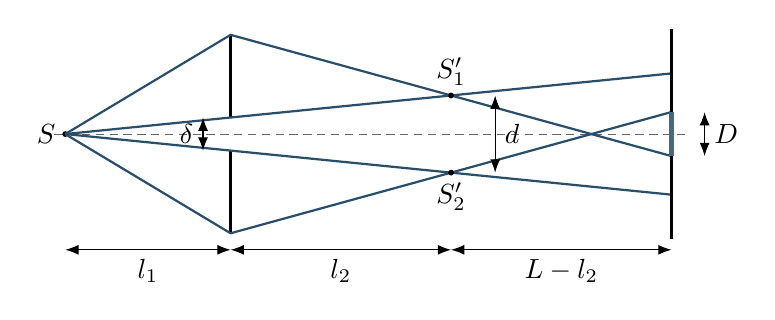
\begin{tikzpicture}[scale=.7,>=Latex]
 \draw[guide](-3.2,0)--(8.3,0);\fill(-3,0)circle(1.5pt)node[left]{$S$};
 \foreach \s in {-1,1}{
  \draw[very thick](0,{\s*.3})--(0,{\s*1.8});\draw[thin](-.12,{\s*.3})--(.12,{\s*.3});
  \foreach \h in {.3,1.8}{\draw[DeepBlue,thick](-3,0)--(0,{\s*\h})--(4,{\s*.7})--(8,{\s*(1.4-\h)});}
  \fill(4,{\s*.7})circle(1.5pt);}
 \draw[very thick](8,-1.9)--(8,1.9);\draw[Blue,line width=2pt](8,-.4)--(8,.4);
 \node[above]at(4,.7){$S_1'$};\node[below]at(4,-.7){$S_2'$};
 \draw[<->](-.5,-.3)--(-.5,.3)node[midway,left]{$\delta$};
 \draw[<->](4.8,-.7)--(4.8,.7)node[midway,right]{$d$};
 \draw[<->](8.6,-.4)--(8.6,.4)node[midway,right]{$D$};
 \draw[<->](-3,-2.1)--(0,-2.1)node[midway,below]{$l_1$};
 \draw[<->](0,-2.1)--(4,-2.1)node[midway,below]{$l_2$};
 \draw[<->](4,-2.1)--(8,-2.1)node[midway,below]{$L-l_2$};
\end{tikzpicture}\figcap{例 21.8 解图：比耶对切透镜、两实像源与公共照明区。竖线是薄透镜所在平面，切口之间留有间隙。}\label{fig:billet}\end{center}}
\newcommand{\MeslinSourceDiagram}{%
\begin{center}\begin{tikzpicture}[scale=.9,>=Latex]
 \draw[guide](-3.2,0)--(6,0);\fill(-3,0)circle(1.5pt)node[left]{$S$};
 \draw[very thick](0,0)--(0,1.5) (2,-1.5)--(2,0);
 \draw[DeepBlue,thick](-3,0)--(0,1.2)--(3,0)--(5,-.8);
 \draw[Blue,thick](-3,0)--(2,-1.2)--({29/7},0)--(5,.48);
 \draw[very thick]({25/7},-1.2)--({25/7},1.2);\fill(3,0)circle(1.5pt);\fill({29/7},0)circle(1.5pt);
 \node[above left]at(3,0){$S_1'$};\node[above right]at({29/7},0){$S_2'$};
 \node[above]at({25/7},1.3){中点屏};\node[below]at(1,-1.7){两半沿轴错开};
 \draw[<->](3,-1.5)--({29/7},-1.5)node[midway,below]{$a$};
 \begin{scope}[shift={(7.4,0)}]
  \foreach \r in {.4,.7,1.0}{\draw[DeepBlue](180:\r)arc[start angle=180,end angle=360,radius=\r];}
  \draw[guide](-1.1,0)--(1.1,0);\node[above]at(0,.2){屏的正视图};
 \end{scope}
\end{tikzpicture}\figcap{例 21.9 解图：梅斯林装置的两像都在光轴上，屏置于两像之间。重叠光只占一侧半屏，条纹为同心半圆弧；轴向间隔已夸大。}\label{fig:meslin}\end{center}}

\newcommand{\NewtonRingsDiagram}{%
\begin{center}\begin{tikzpicture}[scale=.92,>=Latex]
 \begin{scope}
  \draw[very thick](-2.5,0)--(2.5,0);
  \draw[very thick,domain=-2.2:2.2,samples=101]plot(\x,{4-sqrt(16-\x*\x)});
  \draw[thick](-2.2,{4-sqrt(16-2.2*2.2)})--(-2.2,1.1)--(2.2,1.1)--(2.2,{4-sqrt(16-2.2*2.2)});
  \fill(0,0)circle(1.3pt)node[below left]{$O$};
  \draw[<->](1.8,0)--(1.8,{4-sqrt(16-1.8*1.8)})node[midway,right=4pt]{$t(r)$};
  \draw[<->](0,-.65)--(1.8,-.65)node[midway,below]{$r$};
  \node[above]at(0,1.15){平凸透镜};\node[below]at(-1.1,-1.15){底板（透明玻璃特例）};
 \end{scope}
 \begin{scope}[shift={(6,0)}]
  \foreach \m in {1,...,7}{\draw[DeepBlue](0,0)circle({.55*sqrt(\m)});}
  \fill(0,0)circle(.06);\node[below]at(0,-1.65){暗环满足 $r_m^2=m\lambda R$};
 \end{scope}
\end{tikzpicture}\figcap{牛顿环的接触几何与暗环半径。球面在 $O$ 与平板相切，$t(r)$ 两端分别落在平板和球面；环半径按平方级次生成。}\label{fig:newton}\end{center}}

\begin{document}
\pagenumbering{arabic}\setcounter{page}{1}\setcounter{equation}{0}
\section*{第 21 讲\quad 波动光学：干涉}
波动光学研究几何光学不能解释的光学性质，其中最典型的是干涉、衍射和偏振。光是电磁波，两束光在同一点相遇时，先叠加的是电场矢量，而探测到的能流却与电场平方的时间平均成正比。正如 $(a+b)^2$ 中除 $a^2+b^2$ 外还有交叉项，多个光场叠加后的总强度一般不等于各自强度的简单相加；能量在空间重新分布，就是干涉。

日常所见的肥皂泡、油膜和镜头镀膜颜色，都要求同一列光先被分开，沿不同光程传播后再在眼睛或探测器处重合。几何光学能确定每束光的路线，却不能判断重合后的明暗和颜色；这些必须由相位关系决定。

按“怎样把同一列光分开”可把常见装置分为两类。Young 双缝、Fresnel 双棱镜和双面镜从同一波面的不同区域产生次级波，称为分波阵面干涉；薄膜和 Michelson 干涉仪利用部分反射、部分透射把一束光的振幅分开，称为分振幅干涉。两类装置的几何结构不同，但计算核心完全相同：列出到观察点的全部传播光程和界面相变，求相位差，再由振幅叠加得到强度。图 21.1 的同心环纹正是几何光路相近、相位结果却随膜厚和波长改变的典型证据。

\historyfigure{newton-rings-20260923.png}{图 21.1：牛顿环的俯视情景：同心环向外逐渐变密。定量几何见本章牛顿环解图。}
\InterferencePhenomenaPanel

\subsection*{两束光干涉的一般关系}

设同频、同偏振的两束单色光在一点产生
\[
 E_1(t)=E_{01}\cos(\omega t+\varphi_1),\qquad
 E_2(t)=E_{02}\cos(\omega t+\varphi_2).
\]
电磁场满足线性叠加，$E=E_1+E_2$。对远长于光周期的探测时间取平均，得到
\begin{equation}
 I=I_1+I_2+2\sqrt{I_1I_2}\cos\Delta\varphi,\qquad
 \Delta\varphi=\varphi_1-\varphi_2.
\end{equation}
最后一项称为干涉项。若 $I_1=I_2=I_0$，则 $I_{\max}=4I_0$、$I_{\min}=0$；若振幅不同，即使相消位置也不能完全变黑。干涉可见度还要求频率相同或带宽足够窄、偏振方向不正交，且相位差在探测时间内稳定。两个互不相关的普通光源相位快速漂移，干涉项平均为零。

上述平均式可从瞬时场逐项看清。展开 $(E_1+E_2)^2$ 后，$\cos^2(\omega t+\varphi)$ 在许多光周期上的平均为 $1/2$，交叉项的平均为 $\tfrac12\cos(\varphi_1-\varphi_2)$；探测器来不及跟随约 $10^{15}\,\mathrm{Hz}$ 的电场振荡，只记录这个时间平均。若定义条纹可见度
\[
 \mathcal V=\frac{I_{\max}-I_{\min}}{I_{\max}+I_{\min}},
\]
则理想同偏振两束光有
\[
 \mathcal V=\frac{2\sqrt{I_1I_2}}{I_1+I_2}.
\]
所以两路亮度越接近，明暗反差越大；“完全相消”不仅要求相位差为 $\pi$，也要求两振幅相等。偏振正交或相位随机时，交叉项消失，即使两束光在空间重合也看不到稳定条纹。

能量守恒并未被干涉破坏。亮处可能达到单束光强的四倍，是因为能流被重新分配。对无吸收的完整干涉装置，把所有出射端口的功率相加，仍等于总入射功率；例如分光镜的一个端口变暗时，另一个端口可以变亮。不能任取一小块屏面就断言其干涉项积分为零。对于包含许多完整周期、包络变化缓慢的双缝图样，亮暗区的交叉项近似相互抵消。干涉改变能流分布，并不创造能量。

光程差 $\Delta\mathcal L$ 与相位差的关系为
\begin{equation}
 \Delta\varphi=\frac{2\pi}{\lambda_0}\Delta\mathcal L,\qquad
 \mathcal L=\int n\,\dd s,
\end{equation}
其中 $\lambda_0$ 是真空波长。除传播光程外，还要计入反射相位。对透明、无吸收介质的正入射或近正入射，按同一切向电场方向比较，从低折射率侧向高折射率侧反射有 $\pi$ 相变，反向反射无此相变。这就是常用的“半波损失”规则；全反射、金属反射及大角度不同偏振的情形应使用相应的菲涅尔反射系数，不能一概套用。不同路线中的传播相位和界面相位必须作为整体比较。

可见光只是电磁谱中的一小段，真空波长大致从紫光的 $400\,\mathrm{nm}$ 延伸到红光的 $700\,\mathrm{nm}$。同一频率的光进入折射率 $n$ 的介质后，频率不变、相速变为 $c/n$，介质波长变为 $\lambda_0/n$；所以几何长度 $l$ 中累积的相位等于真空中长度 $nl$ 的相位，这就是光程 $nl$ 的由来。比较两路相位时必须统一使用真空波长与光程，或分别使用各介质波长与几何程，不能把两套写法混在同一式中。

\subsection*{Young 双缝：分波阵面干涉}

Young 实验用初级狭缝 $S$ 同相照亮 $S_1,S_2$，从同一波面上取出两个相干次级波源。两缝间距为 $d$，屏距为 $L$，屏上点 $P$ 与主轴夹角为 $\theta$。两路几何程差
\[
 \Delta r=r_2-r_1,\qquad
 \Delta\varphi=\frac{2\pi}{\lambda}\Delta r.
\]
远场条件 $L\gg d$ 且观察角不大时，
\begin{equation}
 \Delta r\simeq d\sin\theta\simeq d\frac yL.
\end{equation}
明纹满足 $\Delta r=m\lambda$，暗纹满足 $\Delta r=(m+1/2)\lambda$，相邻明纹间距
\begin{equation}
 \Delta y=\frac{\lambda L}{d}.
\end{equation}
改变两缝的相对初相位只会平移图样，不改变斜率 $\dd\Delta r/\dd y$，所以条纹间距不变。Young 实验不仅确立了光的波动性，其“路径不可区分时振幅相加”的结构也成为量子物理的重要原型。

远场近似可以从精确距离展开得到。若两缝坐标为 $\pm d/2$，屏点坐标为 $(L,y)$，则
\[
 r_{1,2}=\sqrt{L^2+(y\mp d/2)^2}.
\]
在 $L$ 远大于 $|y|,d$ 时，用 $\sqrt{1+u}=1+u/2+O(u^2)$，有
\[
 r_1\simeq L+\frac{(y-d/2)^2}{2L},\qquad
 r_2\simeq L+\frac{(y+d/2)^2}{2L}.
\]
两式相减得 $r_2-r_1\simeq yd/L$，正负号与前面的定义一致：$y>0$ 时，下缝到观察点更远。再用 $y/L\simeq\sin\theta$ 得到上式。被略去的高阶项会改变远离主轴的条纹间距，因此 $\Delta y=\lambda L/d$ 不是任意近屏、大角度几何下的精确公式。

图 21.3 中初级狭缝 $S$ 不是装饰。若直接用两个彼此独立的灯照亮 $S_1,S_2$，两灯相位各自漂移，屏上的交叉项会在观察时间内平均掉；让同一束光先通过 $S$，再同时照亮两缝，才能获得稳定的相位关系。若 $S$ 到两缝距离不同，只会在 $S_1,S_2$ 间加入固定初相位差 $\varphi_0$，屏上明纹位置变为
\[
 d\frac yL+\frac{\lambda\varphi_0}{2\pi}=m\lambda,
\]
条纹整体平移而间距仍为 $\lambda L/d$。

激光相干长度长、方向性强，图 21.4 中条纹通常清晰且可延伸较远；普通宽带光源的不同波长分别形成不同间距的条纹，只有零光程差附近能够同时保持高可见度。源缝变宽还会把来自不同源点、位置略有错开的条纹叠加，从而降低反差。这些实验条件解释了为什么“有两条光路”只是必要条件，不是出现清晰干涉的充分条件。

\YoungPanel
\YoungPatternPanel

\subsection*{分振幅干涉与薄膜}

分波阵面装置把一个波面的不同区域变成次级波源；分振幅装置则由部分反射/透射把同一束光的振幅分开，再使各束重合。薄膜反射是最常见的分振幅干涉。

图 21.6 中，折射率为 $n$、厚度为 $D$ 的膜置于空气中，入射角为 $i$、膜内折射角为 $r$。上下表面两束反射光的传播光程差为
\[
 \Delta\mathcal L_{\rm geom}=2nD\cos r.
\]
若两次反射中恰有一次发生半波损失，总相位差可写成
\begin{equation}
 \Delta\varphi=\frac{2\pi}{\lambda_0}(2nD\cos r)+\pi.
\end{equation}
因此在\textbf{反射光}中，带一次半波损失时，暗纹满足 $2nD\cos r=m\lambda_0$，明纹满足 $2nD\cos r=(m+1/2)\lambda_0$。若零次或两次相变，明暗条件互换。正入射时只需令 $\cos r=1$。

图 21.6 中传播光程差可逐段核算。进入薄膜的一束在膜内往返的光程为 $2nD/\cos r$；与此同时，直接在上表面反射的另一束在膜外多走了一段，其在出射方向上的投影光程为 $2D\tan r\sin i$。利用 $\sin i=n\sin r$，两者相减：
\[
 \frac{2nD}{\cos r}-2D\tan r\sin i
 =2nD\cos r.
\]
因此 $2nD/\cos r$ 不是最终程差，漏减外部补偿段会把角度依赖写反。相位突变应在传播光程算完后另行加入：只有上下两次反射的相变次数相差奇数，才等效多出 $\lambda_0/2$。

对楔形膜或缓慢变厚的油膜，$D$ 随位置变化，等光程差的位置形成条纹；对白光，不同 $\lambda_0$ 的加强位置不同，于是出现颜色。若膜厚超过光源相干长度，来自不同往返路径的相位关系不再稳定，彩纹会被平均掉。薄膜现象图和薄膜光路图中膜的两个界面、两束最终平行的出射光以及一次相变的位置，必须同时参与判断。

\FilmPhenomenaPanel
\ThinFilmDiagram

太阳能电池、眼镜和相机镜头的增透膜利用反射光相消。取空气、透明膜、透明基底三个介质，折射率满足 $n_0<n_{\rm f}<n_{\rm s}$；正入射时上下界面的反射均有 $\pi$ 相变，二者的相对界面相位为零。要使传播相位相差 $\pi$，最薄的膜须满足 $2n_{\rm f}D=\lambda_0/2$，即 $D=\lambda_0/(4n_{\rm f})$。

\begin{center}\begin{tikzpicture}[>=Latex,font=\small]
\fill[Blue!10](-3,-.6)rectangle(3,.6);
\fill[SoftGray](-3,-1.5)rectangle(3,-.6);
\draw[thick](-3,.6)--(3,.6) (-3,-.6)--(3,-.6);
\node[anchor=west]at(3.3,1.1){空气 $n_0=1$};
\node[anchor=west]at(3.3,0){膜 $n_{\rm f}=1.45$};
\node[anchor=west]at(3.3,-1.1){基底 $n_{\rm s}=3.5$};
\draw[DeepBlue,->](-1.4,1.8)--(-1.4,-.6);
\draw[Blue,->](-.8,.6)--(-.8,1.8);
\draw[Gold,->](.3,-.6)--(.3,1.8);
\node[above]at(-1.4,1.8){入射};\node[above]at(-.5,2.3){两界面反射};
\draw[<->](2.6,-.6)--(2.6,.6)node[midway,left]{$D$};
\end{tikzpicture}\figcap{增透膜的三介质模型。正入射光线为便于辨认而横向分列，实际往返光路重合。}\label{fig:coating}\end{center}

例如 $\lambda_0=550\,\mathrm{nm}$、$n_{\rm f}=1.45$ 时，$D\approx94.8\,\mathrm{nm}$。图~\ref{fig:coating} 的无吸收模型中，未镀膜反射率为 $[(n_{\rm s}-n_0)/(n_{\rm s}+n_0)]^2\approx30.9\%$；计入膜内全部往返反射，四分之一波膜的反射率为
\[
 R=\left(\frac{n_0n_{\rm s}-n_{\rm f}^2}{n_0n_{\rm s}+n_{\rm f}^2}\right)^2\approx6.22\%.
\]
只有 $n_{\rm f}^2=n_0n_{\rm s}$ 时理想反射率才恰为零。这里的基底折射率仅为计算模型；真实硅等材料还具有吸收与色散，不能直接拿此结果替代实测。真实多层膜还要匹配入射角和宽谱响应。镜头表面呈紫红或绿色，是其余波段反射光的综合色。

四分之一波厚度只保证两束主要反射光相差 $\pi$，要做到完全相消还需要两束反射振幅相等。单层膜在正入射下的理想振幅匹配要求膜折射率约为两侧折射率的几何平均；现实材料未必恰好满足，因此反射率只能被显著压低而非严格为零。入射角或波长改变时，$2nD\cos r$ 也随之改变，所以为某一中心波长设计的膜在反射光中会显出其余颜色，多层膜则用多组厚度扩大有效波段。

反射光与透射光的明暗条件互补：忽略吸收时，某波长在反射方向被相消，能量便主要进入透射方向。增透膜并不是把这部分光“吸收掉”，而是利用相位把能流重新分配；高反膜则反过来设计多层界面，使目标波段的反射振幅同相叠加。

\subsection*{Michelson 干涉仪}

Michelson 干涉仪用半透半反分光镜把光分入两条近乎正交的臂，经 $M_1,M_2$ 反射后再次合束。补偿板 $P$ 使两束光穿过相同厚度的玻璃。把一面反射镜关于分光镜成像，两臂等效为两面几乎平行或略有夹角的镜；微小位移会让干涉条纹移动。

若某臂反射镜移动 $x$，往返光程改变 $2x$，每改变一个波长就有一条条纹扫过固定点。这使 Michelson 装置成为高灵敏位移和波长测量工具。Michelson 的工作获 1907 年 Nobel 物理学奖；现代大型激光干涉仪沿用相同相位测量思想，通过长臂、多次反射、真空和隔振检测极小长度变化，引力波探测是其著名应用。

大型引力波装置可以看作把这一原理推到极端：两条互相垂直的真空臂长达千米，光在臂腔中多次往返以增加等效光程，隔振与双站符合则用来排除局部扰动。引力波通过时，两臂长度以相反方式产生极微小相对变化，合束处的相位和光强随之改变。它测量的不是镜子“被光推着移动”，而是两条光路长度差的时间变化；这一区别也说明 Michelson 图中两臂、分光镜、反射镜和探测端的连接关系都不能省略。

分光镜使一路先反射后透射，另一路先透射后反射；若没有补偿板，两路穿过玻璃的次数和厚度不同，宽带光中会出现额外色散，零光程差难以同时满足。把反射镜 $M_2$ 关于分光镜作虚像后，仪器可等效为两面“虚镜”形成的空气薄膜：虚镜平行时得到等倾圆纹，略有夹角时得到近似直条纹。镜移动 $\lambda/2$ 会使往返程差变化一个波长，因此固定点恰有一条纹通过，这是后面例题 21.10 速度测量的直接依据。

\MichelsonDiagram

激光干涉引力波天文台（LIGO）在美国汉福德和利文斯顿各设一台干涉仪，每台的两条真空臂几何长度均为 $4\,\mathrm{km}$。图~\ref{fig:ligo-sites} 中左侧为干旱地区的汉福德站，右侧为森林地区的利文斯顿站；每站两臂互相垂直。不同站点的环境扰动通常不相关，比较两站信号到达时间和波形，是判断天体来源的重要步骤。

\historyfigure{ligo-two-sites-20260923.png}{引力波双站的环境与两条正交长臂；情景图不用于量取尺寸。\label{fig:ligo-sites}}

\begin{center}\begin{tikzpicture}[x=.19cm,y=.13cm,font=\small]
\draw[RuleGray](-125,25)rectangle(-65,50);
\foreach \x in {-120,-100,-80}{\draw[RuleGray](\x,25)--(\x,50);\node[below]at(\x,25){$\x^\circ$};}
\foreach \y in {30,40,50}{\draw[RuleGray](-125,\y)--(-65,\y);\node[left]at(-125,\y){$\y^\circ$};}
\coordinate(H)at(-119.407,46.455);\coordinate(L)at(-90.774,30.563);
\fill[DeepBlue](H)circle(2pt);\fill[DeepBlue](L)circle(2pt);
\draw[Blue,dashed](H)--(L);
\node[above right]at(H){汉福德（美国西北部）};
\node[above right]at(L){利文斯顿（美国南部）};
\end{tikzpicture}\figcap{双站近似经纬位置；横坐标是东经有向角，负值表示西经，纵坐标为北纬。图上直线不用于量取球面距离。}\label{fig:ligomap}\end{center}

图~\ref{fig:ligomap} 中汉福德位于利文斯顿的西北方向。两站具有不同的局部环境，远距离布置使共同信号与单站噪声的区分更有依据；信号到达的先后还取决于波源方向。

首次直接探测到的引力波信号于2015年9月14日到达两站。若应变的量级为 $h\sim10^{-21}$，则单臂长度变化的量级是 $hL\sim4\times10^{-18}\,\mathrm m$，而不是毫米或纳米。臂内的法布里--珀罗腔使光反复往返，低频相位响应约增强300倍；这是光学响应的增强，不能把实体臂长写成几百倍的 $4\,\mathrm{km}$，也不能把增强系数不加频率条件地视为常数。

\MovingLloydPanel

\begin{origexamplebox}{例题 21.1【移动光源】}
Young 双缝实验中，单色点光源沿垂直于主轴方向向上移动一小段，屏上条纹如何变化？A. 上移、间距不变；B. 上移、间距变大；C. 下移、间距不变；D. 下移、间距变大。
\end{origexamplebox}
\begin{xesolution}
光源上移后，到上缝的距离变短、到下缝的距离变长，两个次级光源获得一个固定初相位差。为了重新满足零光程差，屏上观察点必须向下移动，以用“下缝到屏更短”的几何程差补偿源端程差。由于光源移动不改变两缝间距 $d$、屏距 $L$ 和波长，$\Delta y=\lambda L/d$ 不变。
\[
 \boxed{\text{C：条纹向下移动，间距不变。}}
\]
进一步设光源到双缝面的距离为 $a$，上移量为 $s>0$，屏坐标 $y$ 向上为正。上、下缝分别在 $d/2,-d/2$，在 $s,d\ll a$、$y,d\ll L$ 的近轴条件下，两条完整路径之差为
\[
 \Delta\mathcal L=
 \left[\sqrt{a^2+(s+d/2)^2}-\sqrt{a^2+(s-d/2)^2}\right]
 +\left[\sqrt{L^2+(y+d/2)^2}-\sqrt{L^2+(y-d/2)^2}\right]
 \simeq\frac{ds}{a}+\frac{dy}{L}.
\]
中央明纹满足 $\Delta\mathcal L=0$，故 $y_0=-Ls/a<0$；相邻明纹满足程差相差 $\lambda$，仍有 $\Delta y=\lambda L/d$。移源图上部画出这种向下补偿的方向；该结论使用近轴近似。
\end{xesolution}

\begin{origexamplebox}{例题 21.3【劳埃德镜（Lloyd's mirror）】}
劳埃德镜长 $l=7.5\,\mathrm{cm}$；点光源 $S$ 离镜面 $d=0.15\,\mathrm{mm}$，距镜左端 $b=4.5\,\mathrm{cm}$；屏与镜垂直，距 $S$ 的水平距离 $L=1.2\,\mathrm m$。$\lambda=6.0\times10^{-7}\,\mathrm m$。求：（1）干涉区；（2）明纹间距；（3）该区第一条暗纹位置。
\end{origexamplebox}
\begin{xesolution}
反射光等效来自镜面对称虚源 $S'$，但反射带来 $\pi$ 相变。连接 $S'$ 与屏上高度 $y$ 的点，其与镜面的交点横坐标为 $x_0=Ld/(y+d)$。要落在有限镜段，须 $b\le x_0\le b+l$，故
\[
 \frac{Ld}{b+l}-d\le y\le\frac{Ld}{b}-d.
\]
代入数值得
\[
 \boxed{1.35\,\mathrm{mm}\le y\le3.85\,\mathrm{mm}}.
\]
两等效源间距为 $2d$，所以
\[
 \boxed{\Delta y=\frac{\lambda L}{2d}=2.40\,\mathrm{mm}}.
\]
由于反射半波损失，几何程差 $2dy/L=m\lambda$ 的位置是暗纹，即 $y_m=m\Delta y$。干涉区内最小的正整数 $m$ 为 $1$，故第一条暗纹在
\[
 \boxed{y=2.40\,\mathrm{mm}}
\]
处。若漏掉反射相变，会把明暗次序完全颠倒。
\end{xesolution}

\begin{origexamplebox}{例题 21.4【劈尖的干涉】}
透明劈尖的尖角为 $\theta$，沿传播方向 $x$ 的最大厚度为 $h$，折射率为 $n(x)=1+bx$（$b>0$）。将斜面理解为许多微小台阶，各台阶的入射、出射面均垂直于 $x$ 轴，忽略台阶边缘的衍射及反射损失。波长 $\lambda$ 的平行光沿 $+x$ 入射，各光线在介质中直线传播。其后紧贴不透明挡板，开有平行于 $z$ 轴的狭缝；缝在 $y$ 方向排列，第一缝位于尖端 $y=0$，该处厚度为零。理想会聚透镜把各缝光汇聚到后焦点，各缝至焦点的其余光程相同。求其余缝的允许坐标，并判断是否可以选择等距的缝，使焦点处各束光同相加强。
\end{origexamplebox}
\begin{xesolution}
图~\ref{fig:wedge} 中，$y$ 是缝沿挡板的坐标，$x_y$ 才是该光线穿过介质的厚度。由尖角几何，$x_y=y\tan\theta$。
\WedgeInterferenceDiagram
相对于同样几何长度的空气，该光线增加的光程为
\[
 \Delta\mathcal L(y)=\int_0^{x_y}[n(x)-1]\,\dd x
 =\int_0^{x_y}bx\,\dd x=\frac b2y^2\tan^2\theta.
\]
物到像的其余光程相等，故各缝要在透镜焦点同相加强，须 $\Delta\mathcal L(y_m)=m\lambda$：
\[
 \boxed{y_m=\cot\theta\sqrt{\frac{2m\lambda}{b}},\qquad m=0,1,2,\ldots}
\]
并受 $x_y\le h$ 限制，即 $0\le m\le bh^2/(2\lambda)$。注意 $[b]=\mathrm m^{-1}$，所以 $\sqrt{\lambda/b}$ 的量纲为长度。

若把每一个相邻整数级次都开成一条缝，则
\[
 y_{m+1}-y_m=\cot\theta\sqrt{\frac{2\lambda}{b}}
 (\sqrt{m+1}-\sqrt m),
\]
间距确实逐渐减小。但题目并未要求所有允许位置都开缝：\textbf{选取部分级次可以得到等距缝列。}
取任意正整数 $q$，只选 $m=qj^2$，就有
\[
 \boxed{y_j=j\cot\theta\sqrt{\frac{2q\lambda}{b}},\quad
 j=0,1,\ldots,\left\lfloor h\sqrt{\frac{b}{2q\lambda}}\right\rfloor.}
\]
此时第 $j$ 条缝的附加光程为 $qj^2\lambda$，与第一缝的相位差为 $2\pi qj^2$，每束仍同相。最小等距间隔对应 $q=1$；至少能开两条缝还要求 $bh^2\ge2\lambda$。这区分了“连续级次不等距”和“选取级次可以等距”两件事。
\end{xesolution}

\PlaneWaveDiagram

\begin{origexamplebox}{例题 21.5【平行光干涉】}
两束波长均为 $\lambda$ 的平行光从屏法线两侧入射，与法线分别成 $\alpha,\beta$。干涉条纹间距为（
A. $\lambda/(\sin\alpha+\sin\beta)$；
B. $\lambda/(\cos\alpha+\cos\beta)$；
C. $\lambda/(\sin\alpha-\sin\beta)$；
D. $\lambda/|\cos\alpha-\cos\beta|$）。
\end{origexamplebox}
\begin{xesolution}
沿屏面移动 $y$，两束平面波的相位分别改变 $k y\sin\alpha$ 与 $-k y\sin\beta$，故相位差梯度为
\[
 \frac{\dd\Delta\varphi}{\dd y}=k(\sin\alpha+\sin\beta).
\]
相位差增加 $2\pi$ 对应一条纹间距：
\[
 \boxed{\Delta y=\frac{\lambda}{\sin\alpha+\sin\beta}}.
\]
对应选项 A。若两光位于法线同一侧，正负号应按波矢在屏面上的投影重新取值，而不能机械使用相加式。
\end{xesolution}

\BiprismDiagram

\begin{origexamplebox}{例题 21.6【Fresnel 双棱镜】}
双棱镜折射率为 $n$，小棱角为 $\alpha$；缝光源到棱镜距离为 $L_1$，屏到棱镜为 $L_2$。（1）求条纹间距；（2）用折射率 $n'$ 的肥皂膜遮住一半，零级条纹移动 $a$，求膜厚。
\end{origexamplebox}
\begin{xesolution}
每半棱镜使近轴光偏转 $\delta\simeq(n-1)\alpha$，两虚源间距
\[
 d=2L_1(n-1)\alpha.
\]
虚源到屏的距离近似 $L_1+L_2$，故
\[
 \boxed{\Delta y=\frac{\lambda(L_1+L_2)}{2L_1(n-1)\alpha}}.
\]
肥皂膜给一路增加光程 $(n'-1)t$。条纹移动 $a$ 对应的原几何程差为 $da/(L_1+L_2)$，补偿条件给出
\[
 \boxed{t=\frac{ad}{(L_1+L_2)(n'-1)}
 =\frac{2aL_1(n-1)\alpha}{(L_1+L_2)(n'-1)}}.
\]
移动方向由哪一半被遮决定；厚度取正值。
\end{xesolution}

\DoubleMirrorDiagram

\begin{origexamplebox}{例题 21.7【Fresnel 双面镜】}
两镜相对共面位置的小夹角 $\alpha=20'$，缝光源到镜交线距离 $R=10\,\mathrm{cm}$，$\lambda=600\,\mathrm{nm}$，屏距镜交线 $L=210\,\mathrm{cm}$。采用图示对称配置：截面上 $O=(0,0)$、光源 $S=(0,R)$、屏为 $x=L$，两镜方向为 $-45^\circ\mp\alpha/2$，反射面朝向光源，尺寸足以接收公共照明区的光线；忽略边缘衍射，两次反射具有相同相位变化。（1）求间距与最多可见条纹数；（2）$R$ 加倍时怎样变化；（3）光源沿 $+x$ 横移 $\delta s$ 时怎样变化。
\end{origexamplebox}
\begin{xesolution}
先统一几何距离。图 21.11 中镜交线的截点为 $O$，屏位于 $x=L$；取光源 $S=(0,R)$，两镜所在直线的方向角分别为 $-45^\circ-\alpha/2$ 与 $-45^\circ+\alpha/2$。这里 $\alpha$ 是两镜相对于共面位置的小夹角。光源关于两镜的像分别为
\[
 S_1'=(-R\cos\alpha,R\sin\alpha),\qquad
 S_2'=(-R\cos\alpha,-R\sin\alpha).
\]
两镜分别形成相干虚源，间距
\[
 d=2R\sin\alpha\simeq2R\alpha.
\]
虚源平面位于 $O$ 后方 $R\cos\alpha$，所以虚源到屏的距离是 $L+R\cos\alpha$，不是 $L$。因此
\[
 \boxed{\Delta y=\frac{\lambda(L+R\cos\alpha)}{2R\sin\alpha}
 \approx1.134\,\mathrm{mm}}.
\]
两束反射光只在共同照明区内形成条纹。取镜面足够宽、外边缘不另行截光的理想情况，图 21.11 中从 $S_1',S_2'$ 经过 $O$ 的边界射线在屏上交于 $y=\mp L\tan\alpha$，故重叠宽度 $W=2L\tan\alpha\approx24.435\,\mathrm{mm}$。两次反射的相位相同，中心为明纹。固定对称图样的亮纹中心满足 $y_m=m\Delta y$，于是
\[
 N_{\rm bright}=2\left\lfloor\frac W{2\Delta y}\right\rfloor+1
 =\boxed{21}.
\]
对应 $m=-10,\ldots,10$；暗纹中心有22条。若题目的“最多”还允许调节两路恒定相位、把条纹在同宽窗口内平移，则亮纹中心的最大数为 $\lfloor W/\Delta y\rfloor+1=22$。这不是当前中心为亮的对称图样的条数。镜面外缘、挡光片或不计边界纹会进一步限制可见数。

$R$ 加倍后，虚源间距加倍，但虚源到屏的距离也改变：
\[
 \Delta y'=\frac{\lambda(L+2R\cos\alpha)}{4R\sin\alpha}
 \approx0.593\,\mathrm{mm},\qquad
 \frac{\Delta y'}{\Delta y}=\frac{L+2R\cos\alpha}{2(L+R\cos\alpha)}.
\]
比例约为0.523，不是严格的一半。理想重叠宽度不变，固定对称图样有41条亮纹中心，允许调相位时最大42条。

最后必须说明“横移”的方向。取光源沿图中 $+x$ 方向移动 $\delta s$，即 $S=(\delta s,R)$。两虚像坐标变为
\[
 \begin{split}
 S_1'&=(-R\cos\alpha-\delta s\sin\alpha,\ R\sin\alpha-\delta s\cos\alpha),\\
 S_2'&=(-R\cos\alpha+\delta s\sin\alpha,-R\sin\alpha-\delta s\cos\alpha).
 \end{split}
\]
到两虚像等距的点满足中垂线方程 $Ry=\delta s\,x$，故中央亮纹在屏上的位移为
\[
 \boxed{\delta y_0=\frac LR\,\delta s}.
\]
在这一坐标约定下是向 $+y$ 移动；若将源的正方向反取，结果的符号也反取。小位移的一阶近似下条纹间距不变，但公共照明区边界也应随新光路检查。量纲上 $\lambda(L+R)/R$ 是长度；$L\gg R$ 时才恢复常见的 $\lambda L/(2R\alpha)$ 近似。
\end{xesolution}


\begin{origexamplebox}{例题 21.8【Billet 对切透镜】}
焦距为 $f$ 的透镜前 $l_1>f$ 处为波长 $\lambda$ 的缝光源，透镜后 $L$ 处为屏，且 $L>l_2=fl_1/(l_1-f)$。透镜沿直径切为两半并沿切口垂直方向对称移开总距离 $\delta>0$。已知屏上的公共重叠区为 $-D/2\le y\le D/2$，关于中央明纹对称。求条纹间距、亮纹中心的条数，并说明只计两侧暗纹之间完整亮带时如何计数。
\end{origexamplebox}
\begin{xesolution}
\BilletSourceDiagram
未切透镜的像距
\[
 l_2=\frac{fl_1}{l_1-f}.
\]
设某半透镜的光轴平移到 $y=c$。相对于它的新光轴，源的物高为 $-c$，像高为 $(-l_2/l_1)(-c)$；换回原光轴，像的坐标为 $c(1+l_2/l_1)=cl_2/f$。取 $c=\pm\delta/2$，两实像源间距
\[
 d=\delta\frac{l_2}{f}.
\]
屏在像面之后时，相干源到屏的距离为 $L-l_2$，所以
\[
 \boxed{\Delta y=\frac{\lambda(L-l_2)}d
 =\frac{\lambda f(L-l_2)}{\delta l_2}}.
\]
图~\ref{fig:billet} 中 $d$ 是两实像源间距，$D$ 是屏上的公共照明宽度，二者不可混用。由中心亮纹位于 $y=0$，亮纹中心 $y_m=m\Delta y$ 必须满足 $|m|\Delta y\le D/2$，所以包括端点的亮纹中心条数是
\[
 \boxed{N_{\rm center}=2\left\lfloor\frac{D}{2\Delta y}\right\rfloor+1}.
\]
若端点不计入，且 $D/(2\Delta y)$ 恰为整数，应去掉这两条端点纹。若“完整亮纹”指相邻两个暗纹之间的整条亮带，则第 $m$ 条的两侧暗纹位于 $(m\pm\tfrac12)\Delta y$，要求 $(|m|+\tfrac12)\Delta y\le D/2$，因此
\[
 \boxed{N_{\rm full}=\max\!\left\{0,\,
 2\left\lfloor\frac{D}{2\Delta y}-\frac12\right\rfloor+1\right\}.}
\]
如何由实际口径确定题给的 $D$？设每半透镜从切口到外缘的有效高度为 $a_p$，取上半片轴高 $c=\delta/2$、入射高度 $h\in[c,c+a_p]$。屏上光线高度为
\[
 Y=\frac{L}{l_2}\frac{cl_2}{f}+\left(1-\frac{L}{l_2}\right)h.
\]
于是上半束覆盖 $[q-sa_p,q]$，下半束覆盖 $[-q,-q+sa_p]$，其中
$q=\frac\delta2(1+L/l_1)$、$s=L/l_2-1>0$。两者交集给出
\[
 \boxed{D=2\max\{0,\min(q,sa_p-q)\}.}
\]
外缘足够宽时才可化为 $D=2q=\delta(1+L/l_1)$；若 $sa_p\le q$，没有非零宽度的共同照明区，不能直接套条纹计数式。这里将恰在边界上的暗纹算作完整亮带的边界。若孔径使边缘光强趋零，实际能分辨的条数还可能更少。只有在允许条纹任意平移并求最大中心数时，才使用 $\lfloor D/\Delta y\rfloor+1$。
\end{xesolution}

\begin{origexamplebox}{例题 21.9【梅斯林干涉（Meslin interference）】}
凸透镜沿直径切开，两半沿光轴错开。轴上单色点源经两半分别成像于 $S_1',S_2'$，观察屏垂直于轴。（1）求条纹形状；（2）$f=30\,\mathrm{cm}$，物到近半透镜 $60\,\mathrm{cm}$，两半错开 $8\,\mathrm{cm}$，$\lambda=500\,\mathrm{nm}$，屏置于两像中点，求近轴条纹尺度。
\end{origexamplebox}
\begin{xesolution}
\MeslinSourceDiagram
图~\ref{fig:meslin} 中两相干像源在同一轴上，屏在两像之间。若只考虑相位条件，等相位差轨迹是同心圆；但上、下半透镜各只透过半个波面。先成像的一束过轴后进入另一半空间，与尚未成像的一束只在该半屏重叠，所以实际可见的是\boxed{\text{同心半圆弧}}，而不是整圈。

近半透镜像距 $v_1=30\times60/(60-30)=60\,\mathrm{cm}$。远半透镜到物的距离 $68\,\mathrm{cm}$，像距 $v_2=30\times68/(68-30)=53.684\,\mathrm{cm}$，按同一原点计其像坐标为 $8+53.684=61.684\,\mathrm{cm}$。两轴上像源间距
\[
 a=1.684\,\mathrm{cm}.
\]
屏位于中点，一束波在过焦点后发散，另一束仍在向焦点会聚；两波面曲率半径分别为 $+a/2$ 与 $-a/2$。近轴径向相位差增量
\[
 \Delta\varphi(r)-\Delta\varphi(0)=\frac{2kr^2}{a}.
\]
相邻圆纹满足
\[
 \boxed{r_{m+1}^2-r_m^2=\frac{\lambda a}{2}
 =4.21\times10^{-9}\,\mathrm{m^2}=0.00421\,\mathrm{mm^2}}.
\]
上式可直接由球面波相位展开解释：屏到两像的轴向距离均为 $a/2$，离轴点到像的距离增加量约为 $r^2/a$。一束已发散，另一束仍会聚，曲率符号相反，故相位差增加量为 $2kr^2/a$。实际相邻圆弧的径向间距为
\[
 \boxed{r_{m+1}-r_m=\frac{\lambda a}{2(r_{m+1}+r_m)}}.
\]
它随半径增大而减小；$\sqrt{\lambda a/2}\approx64.9\,\mu\mathrm m$ 是平方半径级差对应的特征尺度，不能不考虑轴上相位就把它当作“第一亮环半径”。过焦点相位和两路恒定相位决定中心明暗，不影响上述相邻级次的平方半径差。
\end{xesolution}

\begin{origexamplebox}{例题 21.10【变化臂长】}
Michelson 干涉仪一臂反射镜以速度 $v$ 匀速平移。（1）$\lambda=600\,\mathrm{nm}$，固定取样窗中的信号频率 $50\,\mathrm{Hz}$，求镜速；（2）用平均波长 $589.3\,\mathrm{nm}$ 的钠黄光，镜速同前，拍频 $5.2\times10^{-2}\,\mathrm{Hz}$，求两谱线波长差。
\end{origexamplebox}
\begin{xesolution}
镜移动 $v\dd t$ 使往返光程改变 $2v\dd t$，故条纹频率 $\nu=2v/\lambda$：
\[
 \boxed{v=\frac{\nu\lambda}{2}=1.50\times10^{-5}\,\mathrm{m/s}=15.0\,\mu\mathrm{m/s}}.
\]
两近邻波长产生的时间频率差
\[
 \Delta\nu=2v\left|\frac1{\lambda_1}-\frac1{\lambda_2}\right|
 \simeq\frac{2v\Delta\lambda}{\bar\lambda^2}.
\]
所以
\[
 \boxed{\Delta\lambda=\frac{\Delta\nu\,\bar\lambda^2}{2v}
 \approx6.02\times10^{-10}\,\mathrm m=0.602\,\mathrm{nm}}.
\]
这里两色的光学频率相差很大，探测器并不是记录光场在光学频率上的拍频，而是先分别得到两列随镜位移变化的低频强度信号，再叠加：
\[
 \cos(2\pi\nu_1t)+\cos(2\pi\nu_2t)
 =2\cos[\pi(\nu_1-\nu_2)t]\cos[\pi(\nu_1+\nu_2)t].
\]
包络的绝对值每隔 $1/|\nu_1-\nu_2|$ 再现一次，故题给拍频取两条纹频率之差，不能再多乘或少乘一个 $2$。两谱线强度不等会降低包络谷的深度，但不会改变其再现周期。
这里 $50\,\mathrm{Hz}$ 与 $5.2\times10^{-2}\,\mathrm{Hz}$ 的量级相差三阶，代入时必须保留指数。
\end{xesolution}

\begin{origexamplebox}{例题 21.11【白光干涉】}
白光通过 Young 双缝后为什么出现彩色条纹且级数很少？为什么这种现象难观察？
\end{origexamplebox}
\begin{xesolution}
中央零级处所有波长程差均为零，叠加成白纹。离开中心后，明纹位置 $y_m=m\lambda L/d$ 随波长不同：紫蓝光靠内、红光靠外，形成彩边。级次增大时，不同波长的不同级条纹互相覆盖，综合色趋于均匀，很快失去可见度。

普通白光的相干长度很短，只有两路光程差接近零时相位关系才稳定；双缝又很窄，亮度低，且源缝、双缝和平衡光路必须精确调整。所以白光条纹只在零光程差附近少量出现，远比激光双缝难观察。
\end{xesolution}

\begin{origexamplebox}{例题 21.12【油膜干涉】}
地面油膜为什么呈五彩斑斓？这说明了什么？
\end{origexamplebox}
\begin{xesolution}
白光照到油膜，上、下表面反射光重新重合。对给定位置和观察角，反射相位差约由 $2nD\cos r$ 加界面半波损失决定；不同波长的加强条件不同，所以反射光只突出某些颜色。油膜厚度和表面坡度随位置变化，颜色也随位置改变。

这说明油层薄到与可见光波长同量级，并且在至少一个相干面积内厚度变化缓慢；同时也直接显示光的波动叠加性质。若油层远厚于白光相干长度，众多反射次序平均后便不会形成清晰彩纹。
\end{xesolution}

\begin{origexamplebox}{例题 21.13【薄膜干涉】}
竖直的未吹泡泡液膜从上到下呈不同颜色，颜色缓慢变化并最终变黑，为什么？
\end{origexamplebox}
\begin{xesolution}
重力使液体向下排流，膜通常上薄下厚；每一高度对应不同 $D$，反射增强的波长不同，因而形成近似水平的等厚彩带。排流继续时，同一高度的厚度随时间减小，颜色便缓慢迁移。

当顶部膜厚降到几十纳米量级，$2nD$ 对全部可见波长都很小；上下表面反射中恰有一次 $\pi$ 相变，两束反射光近乎相消，形成“黑膜”。黑色不是液体变黑，而是可见反射光被压低；膜已经很薄，但黑膜可因表面力而维持一段时间，变黑本身不等于已经破裂或必将立即破裂。
\end{xesolution}

\NewtonRingsDiagram

\begin{origexamplebox}{例题 21.14【Newton 环】}
把凸面半径为 $R$ 的平凸透镜以凸面向下放在平面镜上，中心恰好接触，从反射方向观察空气膜的明暗同心环。（1）求第 $m$ 级条纹半径；（2）判断中心明暗；（3）说明这一现象的早期观察者。原题只写“平面镜”，未指定其反射镀层；请先说明所需的反射相位条件，再给出常用透明玻璃底板模型的结果。
\end{origexamplebox}
\begin{xesolution}
“平面镜”只确定几何形状，未确定反射相位。如果是金属镀层，不能从题给的 $R,\lambda$ 唯一确定中心明暗。下面保留一般相位 $\delta_r$，并把透明玻璃底板作为条件明确的特例。
离中心半径 $r$ 处的空气膜厚度由球面几何给出
\[
 t=R-\sqrt{R^2-r^2}\simeq\frac{r^2}{2R}.
\]
图中的 $O$ 是真实接触点，厚度从 $O$ 向外增大。透明玻璃模型下，玻璃到空气的反射无半波损失，空气到玻璃的反射有半波损失，故反射暗环满足 $2t=m\lambda$：
\[
 \boxed{r_m^{(\rm dark)}=\sqrt{m\lambda R},\qquad m=0,1,2,\ldots}
\]
反射明环满足 $2t=(m+1/2)\lambda$：
\[
 \boxed{r_m^{(\rm bright)}=\sqrt{\left(m+\tfrac12\right)\lambda R}}.
\]
$r=0$ 处几何程差为零但有半波损失，因此\boxed{\text{中心为暗纹}}。若透镜与平面不真正接触，中心会因残余膜厚而改变。

如果底板改为金属镜，反射系数一般为复数。设两束反射引入的相对相位为 $\delta_r$，则总相位差为 $4\pi t/\lambda+\delta_r$，相消位置满足
\[
 \frac{4\pi t}{\lambda}+\delta_r=(2m+1)\pi.
\]
在 $r\ll R$ 下，极小与极大的平方半径分别为
\[
 r_{m,\min}^2=\lambda R\left(m+\frac12-\frac{\delta_r}{2\pi}\right),\qquad
 r_{m,\max}^2=\lambda R\left(m-\frac{\delta_r}{2\pi}\right),
\]
只保留右端非负的整数 $m$。中心强度为 $I(0)=I_1+I_2+2\sqrt{I_1I_2}\cos\delta_r$。所以中心是否为暗纹要由 $\delta_r$ 决定，不能直接沿用透明玻璃的半波损失判断；两束振幅不等时，相消处也只是极小而不是完全无光。几何关系 $t\simeq r^2/(2R)$ 仍成立。

这类颜色和环纹在牛顿之前已由罗伯特·胡克（Robert Hooke）观察并记载；牛顿后来作了系统、定量研究，“牛顿环”由此得名。
\end{xesolution}

\end{document}
